% Existing one-shot/comparator measurements are retained at table precision in
% ../data/manuscript_comparators.csv; new trajectories: ../data/graphics_results.csv.
\begin{figure*}[t]
  \centering
  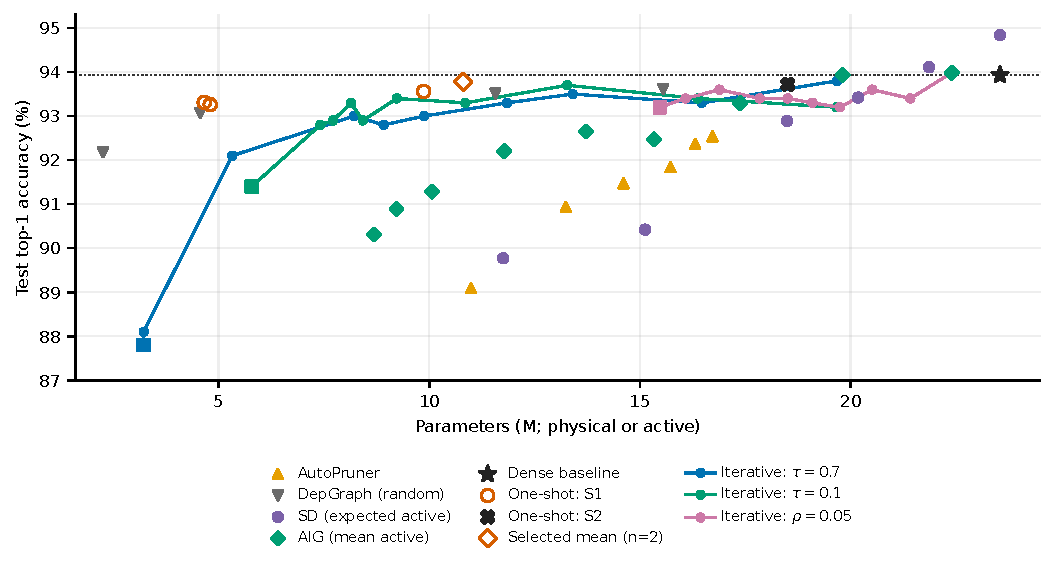
\includegraphics[width=\textwidth]{figures/resnet50_cifar10_selected.pdf}
  \caption{ResNet-50 on CIFAR-10. Fixed networks: the existing one-shot
    results, all 30 iterative channel-pruning models, AutoPruner and
    DepGraph (random importance). Lines follow cycle order and squares
    mark final iterative models. The hollow diamond is a coordinate-wise
    mean of two selected same-seed runs out of eight; it is not a deployed
    network. Dynamic baselines retain the full backbone: AIG counts
    are validation means and SD counts are expectations. Training budgets
    and historical accuracy aggregation differ.}
  \label{fig:resnet-cifar-tradeoff}
  \Description{One plot compares three iterative ResNet channel-pruning
    trajectories, the one-shot models, structural-pruning comparators and
    dynamic baselines, using physical or active parameter counts.}
\end{figure*}

\paragraph{One-shot pruning.}
Figure~\ref{fig:resnet-cifar-tradeoff} and Table~\ref{tab:resnet-cifar-all}
show the trade-off between accuracy and model size for ResNet-50 on
CIFAR-10. The dense
baseline achieves 93.93\% test accuracy with 23.547M parameters.

Our 4.660M-parameter model achieves 93.31\% accuracy, reducing the
parameter count by 80.2\% with an accuracy loss of 0.62 percentage points.
The nearest DepGraph model achieves 93.07\% with 4.566M parameters.
Our model therefore achieves 0.24 percentage points higher accuracy
with 2.1\% more parameters.

Averaging two selected repeats gives 10.805M parameters and
93.78\% accuracy, corresponding to 54.1\% fewer parameters and an
accuracy gap of 0.15 percentage points from the dense baseline.
The nearest DepGraph model achieves 93.51\% with 11.569M parameters.

Stochastic Depth reaches up to 94.84\% accuracy but retains all
23.547M parameters in storage.

\paragraph{Iterative channel pruning.}
Three channel-pruning trajectories in
Figure~\ref{fig:resnet-cifar-tradeoff} contain ten
models each, ordered by cycle rather than by notebook row order.
The threshold series $\tau=0.7$ reaches 92.1\% at 5.325M
parameters before declining to 87.8\% at 3.220M in its final
model. The $\tau=0.1$ series ends at 91.4\% with 5.787M
parameters. The budget-only series $\rho=0.05$ retains 15.475M parameters with
93.2\% accuracy at the end. Complete trajectories are given in
Table~\ref{tab:resnet-notebook-trajectories}.

\paragraph{Block pruning.}
Four historical block-pruning models in Figure~\ref{fig:additional-pruning-trajectories}(b) span 15.266--18.974M parameters and 92.80--93.27\%
reported accuracy. Their final and preceding recovery models
have the same parameter count but different accuracies;
they are separate checkpoints, not seed repetitions.

% Existing rows retain their previously reported precision and accuracy changes.
% Generated by paper/scripts/build_results.py from graphics_results.csv.

\newcommand{\ResNetIterativeFinalRows}{%
$\tau=0.7$ & 3.220 & 13.7 & 87.8 & -6.13 \\
$\tau=0.1$ & 5.787 & 24.6 & 91.4 & -2.53 \\
$\rho=0.05$ & 15.475 & 65.7 & 93.2 & -0.73 \\
}

\begin{table*}[t]
  \caption{ResNet-50/CIFAR-10 one-shot and comparator results, with the three
    final iterative channel-pruning models. All 30 iterative checkpoints
    are listed in Table~\ref{tab:resnet-notebook-trajectories}. Params: reported parameter
    count (M) and its share of the dense model (23{,}547{,}338 parameters,
    \%). $\Delta$: accuracy difference from the Baseline in percentage
    points. S1 and S2 denote our two sweeps; the following pair gives
    $\delta_s/\delta_h$ in percentage points. Mean averages both
    coordinates of two selected runs from eight same-configuration,
    same-seed repeats; it is not one deployed network.
    Iterative settings use threshold $\tau$ or budget fraction $\rho$.
    DepGraph settings are target FLOPs speedups; $k$ is AutoPruner's
    target keep ratio, $p_L$ the final survival probability, and $t$
    the ConvNet-AIG target rate. $\dagger$: expected active parameters
    under stochastic inference; $\ddagger$: active parameters averaged
    over validation images. Both marked methods retain the full backbone
    weights. Training budgets and historical accuracy aggregation differ.}
  \label{tab:resnet-cifar-all}
  \centering
  \small
  \setlength{\tabcolsep}{4pt}
  \begin{minipage}[t]{0.48\textwidth}
    \centering
    \begin{tabular}[t]{@{}lrrrr@{}}
      \toprule
      Setting & Params (M) & \% & Acc. (\%) & $\Delta$ \\
      \midrule
      \multicolumn{5}{l}{\textit{Baseline}} \\
      % 716de1ac4ae743689a7962a3a4dfae3b
      dense & 23.547 & 100.0 & 93.93 & 0.00 \\
      \midrule
      \multicolumn{5}{l}{\textit{Ours: one-shot (selected)}} \\
      % resnet50_cifar10_ls0_curve7_v1/large_18m
      S1: $0.025/0.05$ & 4.660 & 19.8 & 93.31 & $-$0.62 \\
      % resnet50_cifar10_ls0_curve7_v1/middle_8m
      S1: $0.25/0.5$ & 4.801 & 20.4 & 93.26 & $-$0.67 \\
      % resnet50_cifar10_ls0_curve7_v1/floor_probe_2p9m
      S1: $5/10$ & 9.868 & 41.9 & 93.56 & $-$0.37 \\
      % resnet50_cifar10_ls0_prebn_repeat8_v1/mean_selected_repeats_05_07
      Mean ($n=2$) & 10.805 & 45.9 & 93.78 & $-$0.15 \\
      % resnet50_cifar10_ls0_curve7_v2/middle_8m
      S2: $0.25/0.5$ & 18.512 & 78.6 & 93.72 & $-$0.21 \\
      \midrule
      \multicolumn{5}{l}{\textit{Ours: iterative (final cycle)}} \\
      \ResNetIterativeFinalRows
      \midrule
      \multicolumn{5}{l}{\textit{DepGraph (random importance)}} \\
      % a66ef23af1d94813bf2629ffec935f40
      $\times1.5$ & 15.554 & 66.1 & 93.62 & $-$0.31 \\
      % ab961d162f4646cb8773ab9f7445607f
      $\times2.0$ & 11.569 & 49.1 & 93.51 & $-$0.42 \\
      % 60622bbe09914eb8aa7a2b0906acf673
      $\times5.0$ & 4.566 & 19.4 & 93.07 & $-$0.86 \\
      % 6839c67c7d974f949927e1deafd78957
      $\times10.0$ & 2.258 & 9.6 & 92.18 & $-$1.75 \\
      \midrule
      \multicolumn{5}{l}{\textit{AutoPruner}} \\
      % AutoPruner keep=0.3
      $k=0.3$ & 10.993 & 46.7 & 89.09 & $-$4.84 \\
      % AutoPruner keep=0.5
      $k=0.5$ & 13.242 & 56.2 & 90.94 & $-$2.99 \\
      % AutoPruner keep=0.6
      $k=0.6$ & 14.612 & 62.1 & 91.47 & $-$2.45 \\
      % AutoPruner keep=0.7
      $k=0.7$ & 15.728 & 66.8 & 91.84 & $-$2.09 \\
      % AutoPruner keep=0.8
      $k=0.8$ & 16.312 & 69.3 & 92.37 & $-$1.55 \\
      % AutoPruner keep=0.9
      $k=0.9$ & 16.722 & 71.0 & 92.54 & $-$1.39 \\
      \bottomrule
    \end{tabular}
  \end{minipage}\hfill
  \begin{minipage}[t]{0.48\textwidth}
    \centering
    \begin{tabular}[t]{@{}lrrrr@{}}
      \toprule
      Setting & Params (M) & \% & Acc. (\%) & $\Delta$ \\
      \midrule
      \multicolumn{5}{l}{\textit{Stochastic Depth}} \\
      % Stochastic Depth p_L=0.3
      $p_L=0.3$ & 11.756$^\dagger$ & 49.9 & 89.77 & $-$4.16 \\
      % Stochastic Depth p_L=0.5
      $p_L=0.5$ & 15.125$^\dagger$ & 64.2 & 90.42 & $-$3.50 \\
      % Stochastic Depth p_L=0.7
      $p_L=0.7$ & 18.494$^\dagger$ & 78.5 & 92.89 & $-$1.04 \\
      % Stochastic Depth p_L=0.8
      $p_L=0.8$ & 20.179$^\dagger$ & 85.7 & 93.42 & $-$0.51 \\
      % Stochastic Depth p_L=0.9
      $p_L=0.9$ & 21.863$^\dagger$ & 92.8 & 94.11 & $+$0.18 \\
      % Stochastic Depth p_L=1.0
      $p_L=1.0$ & 23.547$^\dagger$ & 100.0 & 94.84 & $+$0.91 \\
      \midrule
      \multicolumn{5}{l}{\textit{ConvNet-AIG}} \\
      % bffb9a169ea949aeb7f6853eb49272f7
      $t=0.1$ & 8.696$^\ddagger$ & 36.9 & 90.31 & $-$3.62 \\
      % 9512a6073f7e41a5adb6758211a6a555
      $t=0.2$ & 9.224$^\ddagger$ & 39.2 & 90.88 & $-$3.05 \\
      % b6b35731d7f74cd8b9ffd790c8b71864
      $t=0.3$ & 10.068$^\ddagger$ & 42.8 & 91.28 & $-$2.65 \\
      % a447cf7d416e49d9a145881241071636
      $t=0.4$ & 11.783$^\ddagger$ & 50.0 & 92.20 & $-$1.73 \\
      % 85ef57c9020e449e83d9b9939fa9d50c
      $t=0.5$ & 13.717$^\ddagger$ & 58.3 & 92.65 & $-$1.28 \\
      % eb38db75adaa43658ba861536699ccc5
      $t=0.6$ & 15.335$^\ddagger$ & 65.1 & 92.47 & $-$1.45 \\
      % 5f97b677390845d7995d4c3f904ee954
      $t=0.7$ & 17.383$^\ddagger$ & 73.8 & 93.29 & $-$0.64 \\
      % 500f50a024014ba4bf57ec7b92d91931
      $t=0.8$ & 19.811$^\ddagger$ & 84.1 & 93.93 & 0.00 \\
      % 1664739e725b4bf0ae0bf87df187ee91
      $t=0.9$ & 22.406$^\ddagger$ & 95.2 & 93.98 & $+$0.05 \\
      \bottomrule
    \end{tabular}
  \end{minipage}
\end{table*}
